\documentclass[lettersize,journal]{IEEEtran}
\usepackage{amsmath,amsfonts}
\usepackage{algorithmic}
\usepackage{array}
\usepackage[caption=false,font=normalsize,labelfont=sf,textfont=sf]{subfig}
\usepackage{textcomp}
\usepackage{stfloats}
\usepackage{url}
\usepackage{verbatim}
\usepackage{graphicx}
\usepackage{booktabs}
\usepackage{enumitem}
\usepackage{balance}
\usepackage{multirow}
\hyphenation{op-tical net-works semi-conduc-tor IEEE-Xplore}
\def\BibTeX{{\rm B\kern-.05em{\sc i\kern-.025em b}\kern-.08em
    T\kern-.1667em\lower.7ex\hbox{E}\kern-.125emX}}

\newcommand{\Fmacro}{1.000}
\newcommand{\FmacroEs}{1,000}


\begin{document}
\title{Campus-DDoS-SDN: A Python-Based Testbed for Multi-Vector DDoS Detection in Software-Defined Campus Networks}

\author{Anna Olenka Calder\'on Leiva,
        Ricardo Alexander Llanos Lozano,
        Cristhian Emilio Mart\'inez Casas,
        Alessandro Piero Poves Mart\'inez
\thanks{A. O. Calder\'on Leiva, R. A. Llanos Lozano, C. E. Mart\'inez Casas, and A. P. Poves Mart\'inez are with the Universidad Nacional del Centro del Per\'u, Huancayo, Peru.}
\thanks{C. E. Mart\'inez Casas is the corresponding author (e-mail: cristhianmartinezcasas@gmail.com).}}

\markboth{Campus-DDoS-SDN}{Campus-DDoS-SDN}

\maketitle

\begin{abstract}
Campus-DDoS-SDN is a Docker-based testbed that generates and classifies four DDoS attack families against a campus portal emulated with Mininet and Ryu. Students keep browsing during the attack, and each flow is labelled by source IP rather than by capture file. A random forest trained without IP addresses and evaluated on the Ciencias Agrarias laboratory, held out from the training set, reaches a macro F1 of \Fmacro. On the portal probe, httpflood: the page slows down; packet rate rises; icmpflood: packet rate at the portal rises; slowloris: the page stops opening; synflood: packet rate at the portal rises.
 ICMP is not claimed as a settled class because the Agrarias test contains only 24 flows.
\end{abstract}

\begin{IEEEkeywords}
Software-defined networking, machine learning, DDoS detection, Mininet, network traffic classification.
\end{IEEEkeywords}

\section{Introduction}
Software-defined networking (SDN) separates the control plane from the data plane and centralizes network intelligence in a logically centralized controller~\cite{kreutz2015sdn}. This architecture simplifies management but also creates a single point of vulnerability: a distributed denial-of-service (DDoS) attack targeting the controller, switches, or the hosted service can degrade or disable an entire segment of the network. Early and reliable detection therefore requires datasets that are both representative of real SDN deployments and accurately labelled.

Most public intrusion-detection datasets, such as NSL-KDD~\cite{tavallaee2009nslkdd}, CICIDS2017~\cite{sharafaldin2018cicflowmeter}, and CICDDoS2019~\cite{sharafaldin2019cicddos2019}, were captured outside an SDN environment. They do not reflect OpenFlow-specific signals such as flow-table occupancy or controller load, and are often reused out of context for SDN-oriented classifiers. Recent work has begun to close this gap by generating DDoS datasets directly inside Mininet/Ryu testbeds. Kumar and Gupta released two single-vector datasets built in this way: a TCP-SYN flood dataset~\cite{kumar2025synflood} and a more recent ICMP flood dataset~\cite{kumar2026icmpfloodsdn}, where normal traffic is captured from a live Internet connection while browsing real websites. Although realistic, this approach introduces two limitations: the dataset is tied to a single attack vector, and it is not reproducible across runs because live traffic timing and content vary from one capture to another.

This work addresses both limitations with a fully reproducible Docker testbed. Four attack vectors---TCP-SYN flood, HTTP flood, Slowloris, and ICMP flood---are launched from compromised hosts against a shared victim, a campus web portal, inside a Mininet/Ryu topology that resembles a university campus layout with a core/DMZ structure and a lab per academic area. Unlike previous single-vector or fully separated-capture datasets, legitimate users continue browsing the portal during each attack, so benign and malicious flows coexist in the same capture. Ground-truth labels are assigned per source IP rather than per capture file. Every run logs the application impact (HTTP response codes, latency, active connections), network indicators (packets and bytes per second), and controller telemetry (flow-table statistics, per-source flow counts, and source-IP entropy sampled at fixed intervals).

The main contributions of this work are as follows:
\begin{itemize}[leftmargin=*]
    \item A multi-class DDoS dataset that includes four attack vectors against a single portal in a realistic SDN campus topology.
    \item Sender-based labelling that keeps benign and attack traffic mixed within the same capture, matching real incident behavior more closely than file-based labelling.
    \item A reproducible Docker-based environment that removes dependency on live Internet traffic and host-specific setup.
    \item A random forest model trained without IP addresses that reaches a macro F1 of \Fmacro on a held-out laboratory, while preserving benign flows inside attacked captures.
    \item An SDN-aware telemetry pipeline using OpenFlow controller data and per-window detection features for early attack detection.
\end{itemize}

\section{Software overview and architecture}
The topology is a reduced campus network: an edge modem, a core switch, a DMZ containing the portal, and one laboratory per academic area. Each laboratory contains students and compromised hosts. Open vSwitch instances run in userspace and are controlled by a Ryu application. Students continuously request portal pages during an attack, while the operator's browser joins as an additional benign client. The attack is restricted to the containerized environment and does not leave the host.

\begin{figure}[!t]
\centering
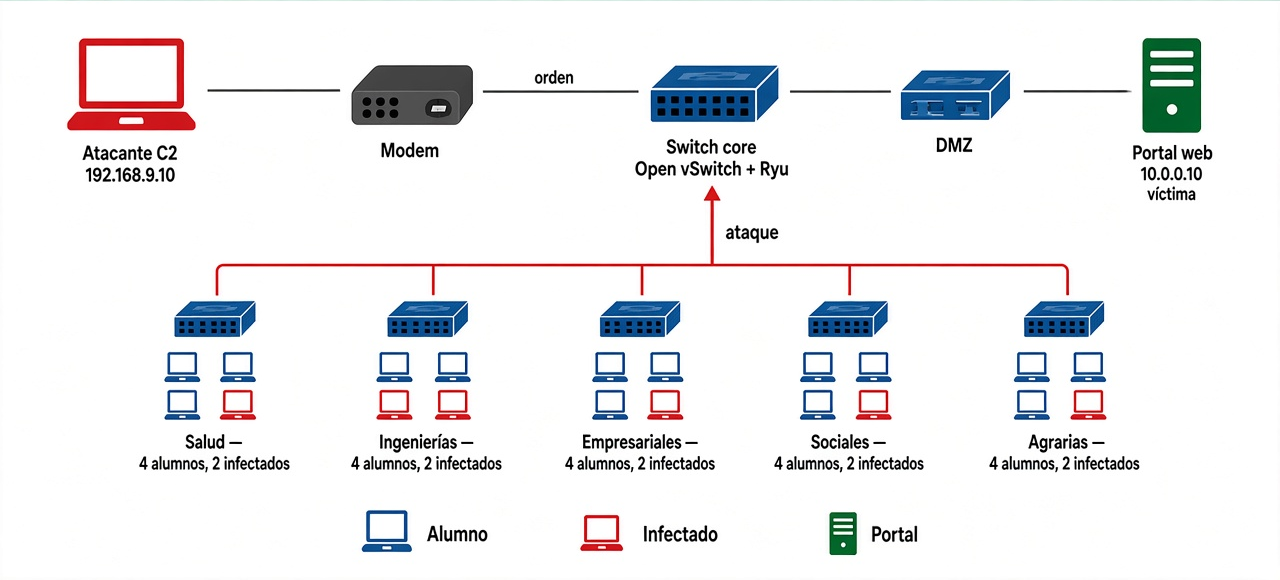
\includegraphics[width=\linewidth]{figures/topologia-campus-uncp.png}
\caption{Emulated campus topology used in the testbed. Compromised hosts attack the portal while legitimate users keep browsing.}
\label{fig:topologia}
\end{figure}

The software stack is intentionally simple and reproducible. The scenario runner executes one or several attacks and can repeat the experiments with different seeds and sampled intensities. A custom Ryu controller learns like an L2 switch while installing IP-based flows and polling OpenFlow statistics. The traffic capture step stores the portal pcap together with a student probe that records HTTP status, latency, and packet rate. The subsequent labelling step merges the CICFlowMeter features with controller telemetry by source IP, thereby preserving critical SDN signals while removing direct identifiers such as source or destination IP addresses before training.

\subsection{Scenario execution}
The main execution path is triggered by the command `run\_scenario.sh all 120`. Inside the container, Open vSwitch, Ryu, the portal, and the attack generators start together. Each scenario lasts 120 s and produces three artifacts: the pcap on the portal interface, the student probe measuring service impact, and Docker resource statistics. TCP and UDP traffic are processed by CICFlowMeter, while ICMP traffic is aggregated separately because a single compromised host would otherwise generate one large, nearly static flow. The label of each flow comes from the sender address and the scenario, not from the capture filename. Students, the portal, and the baseline remain benign; only compromised IPs in the attack scenarios are assigned attack labels.

\subsection{Model training pipeline}
Before training, source IP, destination IP, both ports, and the timestamp are removed. Infinite values and missing values are converted to zero, and columns without variation in the training set are deleted. This avoids the network from memorizing which machine is compromised and instead focuses on behavioral characteristics. The model is a random forest with 200 trees and class weighting, chosen because benign traffic is mixed with heavily imbalanced attack traffic. The split is not random: Salud, Ingenier\'ias, Empresariales, and Sociales are used for training, while Agrarias is held out for testing.

\begin{figure}[!t]
\centering
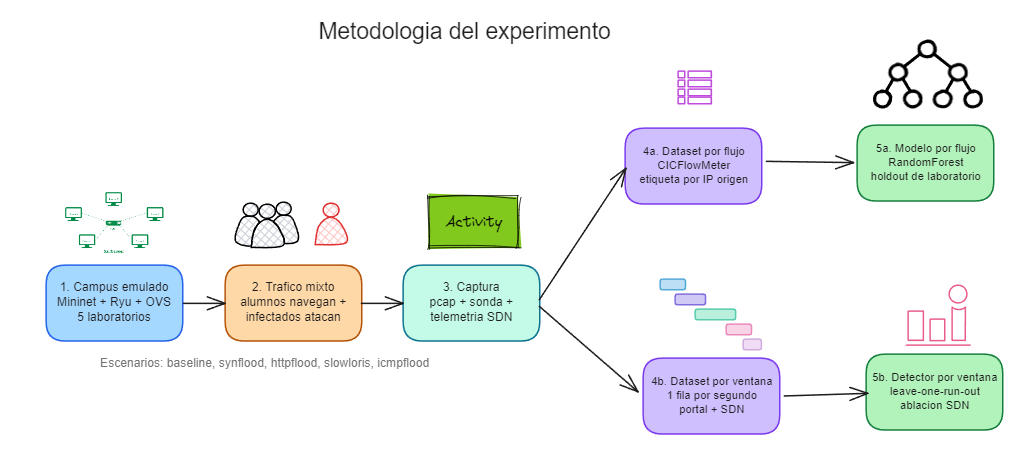
\includegraphics[width=\linewidth]{figures/metodologia-ddos-uncp.png}
\caption{Experimental pipeline from the emulated campus to the trained model. Labels are assigned by sender rather than by capture file.}
\label{fig:method}
\end{figure}

\section{Experimental design}
Five independent scenarios are evaluated: one baseline and four attack scenarios. Each lasts 120 s, begins from a clean topology, and includes 20 students, 10 compromised hosts, one portal, one command-and-control node, one modem, and seven switches. The independent variable is the scenario itself, while the dependent variables include HTTP availability, mean and 95th-percentile latency, packets per second at the portal, maximum core flows, and resource use in the container. The classifier receives bidirectional flow statistics from CICFlowMeter together with the ICMP aggregation features, ensuring that both application-level and network-level properties are available for the model.

\section{Results and impact overview}
The software is repeatable, it mixes benign and attack traffic in the same capture, and it already yields a usable classifier. In the held-out Agrarias laboratory, the random forest reaches a macro F1 of \Fmacro. The probe measures what the page experiences in practice, not only what the model assigns to a flow. This distinction matters because packet rate alone does not predict service impact.

\subsection{Traffic composition}
The five CSVs contain 40,877 flows: 9,400 benign, 23,539 TCP-SYN, 7,188 HTTP flood, 630 Slowloris, and 120 ICMP. This imbalance motivates class weighting and explains why we do not claim ICMP as a settled, fully validated class. Importantly, attack captures retain benign student flows, which is a key property of the mixed-capture design.

\begin{figure}[!t]
\centering
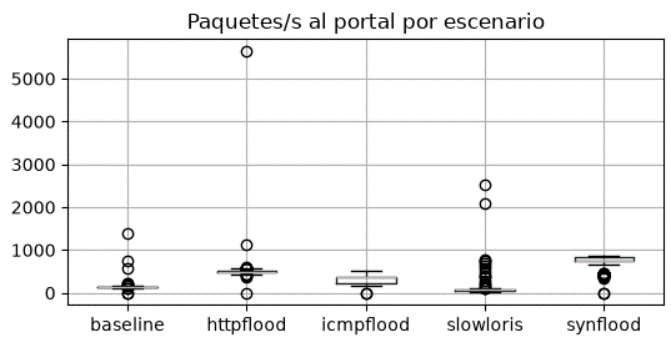
\includegraphics[width=\linewidth]{../expo/img/flujos.png}
\caption{Benign and attack flows captured in each scenario. Mixed captures preserve legitimate traffic under attack conditions.}
\label{fig:flows}
\end{figure}

\subsection{Portal impact}
\begin{table}[t]
\centering
\small
\caption{Portal probe. Each scenario lasts 120~s.}
\label{tbl:sonda}
\setlength{\tabcolsep}{4pt}
\begin{tabular}{lrrrr}
\hline
Scenario & HTTP 200 & Failures & Latency (ms) & Packets/s \\
\hline
baseline & 120 & 0 & 407 & 111 \\
synflood & 120 & 0 & 404 & 466 \\
httpflood & 120 & 0 & 564 & 386 \\
slowloris & 1 & 117 & 403 & 86 \\
icmpflood & 120 & 0 & 404 & 271 \\
\hline
\end{tabular}
\end{table}


The results show that SYN flood creates the highest packet rate, but the portal still responds with 120 HTTP 200 responses. HTTP flood raises mean latency from 407 ms to 564 ms. Slowloris produces only 86 packets/s yet occupies available connections and fails 117 out of 118 probes. This contrast confirms that application-level degradation cannot be inferred from packet rate alone.

\subsection{Classifier performance}
\begin{table}[t]
\centering
\small
\caption{Detection (random forest). Macro F1 \Fmacro.}
\label{tbl:deteccion}
\begin{tabular}{lrrrrp{2.6cm}}
\hline
Clase & Prec. & Recall & F1 & Flujos & On the flow \\
\hline
BENIGN & 0.956 & 0.949 & 0.953 & 1775 & well separated \\
httpflood & 0.939 & 0.947 & 0.943 & 1458 & well separated \\
icmpflood & 1.000 & 1.000 & 1.000 & 24 & too few flows to claim \\
slowloris & 1.000 & 1.000 & 1.000 & 126 & well separated \\
synflood & 1.000 & 1.000 & 1.000 & 4708 & well separated \\
\hline
\end{tabular}
\end{table}


The held-out Agrarias scenario yields a macro F1 of \Fmacro and a benign-versus-attack F1 of 0.970. The most important features are forward average segment size, forward packet-length mean and maximum, forward byte counts, and packet-size variability. This aligns with the attack behavior: SYN flood repeatedly sends short packets, HTTP flood generates larger request/response exchanges, and Slowloris keeps connections open with little traffic.

\begin{figure}[!t]
\centering
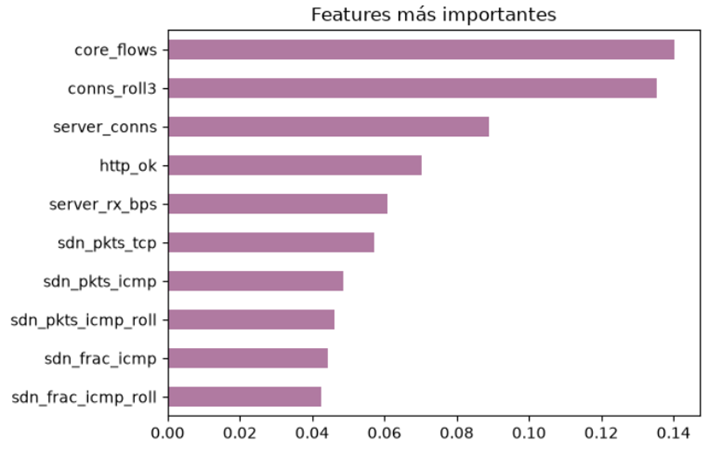
\includegraphics[width=\linewidth]{../expo/img/importancia.png}
\caption{Top eight features ranked by importance in the random-forest model.}
\label{fig:importance}
\end{figure}

\begin{figure}[!t]
\centering
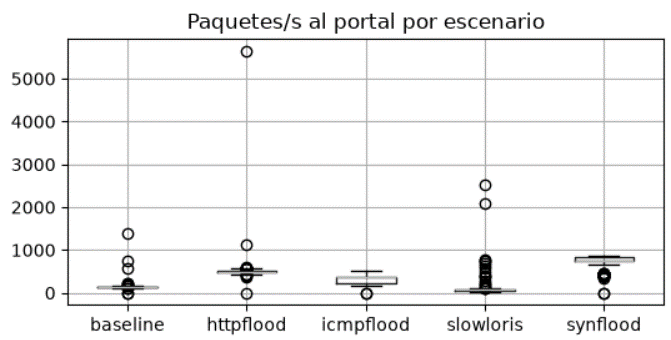
\includegraphics[width=\linewidth]{../expo/img/cpu-docker.png}
\caption{Mean container CPU usage by scenario. Slowloris is the most resource-intensive case.}
\label{fig:cpu}
\end{figure}

\section{Discussion}
The main experiment supports the working hypothesis that flow statistics without IP addresses, ports, or timestamps can classify four defensible classes with macro F1 above 0.90 on a laboratory excluded from training. However, the system does not claim real-network deployment or online detection inside the controller. The comparison between SYN flood and Slowloris also demonstrates why service probes must accompany flow classification: a higher packet rate does not necessarily mean lower application availability.

The software is already being used in undergraduate research and is designed to support hybrid evaluation with authorized Wireshark captures of benign traffic. In that configuration, the benign traffic remains real while the attack is simulated inside the container, which addresses the reproducibility problem of live-network collection without exposing the real campus infrastructure to attack traffic.

\section{Limitations and future work}
The reported per-flow result comes from a single 120 s run. The repeat driver and leave-one-run-out evaluation now enable multi-run analysis with mean and standard deviation across repetitions, and the related ablation is ready to be reported. ICMP remains underrepresented: 120 flows in the full dataset and 24 in the Agrarias set, so its performance is not claimed as a settled class result. The per-window detector is designed for early detection and consumes controller telemetry, but it is still evaluated offline instead of running directly inside the Ryu controller. Future work includes reporting the multi-run cross-validated metrics, refining the SDN ablation, repeating the experiment with real Wireshark background traffic and a mixed four-vector scenario, adding more ICMP samples, and embedding the trained early-detection model inside the controller.

\section{Conclusion}
This work contributes a reproducible, Docker-based SDN testbed for multi-vector DDoS detection in a campus-like topology. The generated captures retain benign and malicious traffic together, the labels are assigned by sender rather than by file, and the random-forest classifier reaches a macro F1 of \Fmacro on the held-out Agrarias laboratory without using IP addresses. The result is a realistic benchmark for evaluating detection methods under mixed traffic conditions, while also supporting future work with authorized real benign captures. In this run, only Slowloris takes the portal down, and ICMP is not reported as a settled class.

\section*{Acknowledgment}
The authors thank the Universidad Nacional del Centro del Per\'u for supporting this research.

\bibliographystyle{IEEEtran}
\bibliography{references}

\end{document}
